\documentclass{article}
\usepackage{tikz,pgfplots}
%\pgfplotsset{colormap={name}{
%	color(0cm)=(blue);
%	color(1cm)=(green);
%	color(2cm)=(yellow)
%	color(3cm)=(red)}}
\pgfplotsset{colormap={blues}{
       color(0cm)=(white);
       color(1cm)=(blue)}}

\definecolor{diplom1}{rgb}{0.0 0.4 1.0}
\definecolor{diplom2}{rgb}{0.0 0.0 0.6}
\definecolor{diplom3}{RGB}{153,0,0} %unirot
\definecolor{diplom4}{RGB}{232,215,23}
\definecolor{diplom5}{RGB}{51,37,60}

\definecolor{unirot}{RGB}{153,0,0}
\definecolor{unirot_hell}{RGB}{255,228,225}
\definecolor{lightblue}{RGB}{242.2,249.88,255}

\begin{document}


   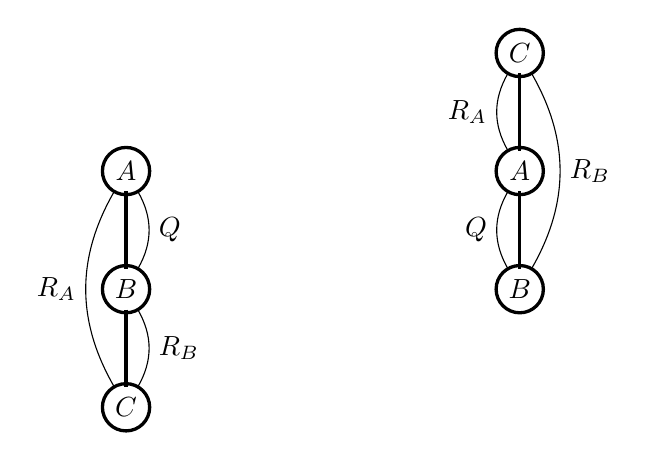
\begin{tikzpicture}[scale=1.0,>=stealth]
%       \draw [help lines] (0,0) grid (10,7);
       
       \draw [very thick] (2,4) circle (0.3)
              node [name=A] {$A$};
       \draw [very thick] (2,2.5) circle (0.3)
              node [name=B] {$B$};
       \draw [very thick] (2,1) circle (0.3)
              node [name=C] {$C$};
       \draw [very thick] (A) -- (B);
       \draw [very thick] (B) -- (C);
       \path (A) edge [bend left] node [right] {$Q$} (B)
             (B) edge [bend left] node [right] {$R_B$} (C)	
             (A) edge [bend right] node [left] {$R_A$} (C);

    \begin{scope}[xshift=5cm]
       \draw [very thick] (2,4) circle (0.3)
              node [name=A] {$A$};
       \draw [very thick] (2,2.5) circle (0.3)
              node [name=B] {$B$};
       \draw [very thick] (2,5.5) circle (0.3)
              node [name=C] {$C$};
       \draw [very thick] (A) -- (B);
       \draw [very thick] (A) -- (C);
       \path (A) edge [bend right] node [left] {$Q$} (B)
             (B) edge [bend right] node [right] {$R_B$} (C)	
             (A) edge [bend left] node [left] {$R_A$} (C);
    \end{scope}

   \end{tikzpicture}



\end{document}
